% Presentation for Lab 2. Build (XeLaTeX, Arial from Windows fonts mounted at /winfonts):
% docker run --rm -v "<project>/docs:/work" -v "C:/Windows/Fonts:/winfonts:ro" -w /work \
%   texlive/texlive:latest-medium latexmk -xelatex presentation.tex
\documentclass[aspectratio=169,11pt]{beamer}

\usepackage{fontspec}
\setsansfont{arial.ttf}[Path=/winfonts/, BoldFont=arialbd.ttf, ItalicFont=ariali.ttf, BoldItalicFont=arialbi.ttf]
\setmonofont{consola.ttf}[Path=/winfonts/, BoldFont=consolab.ttf, Scale=0.92]
\usepackage{booktabs}
\usepackage{array}
\newcolumntype{L}[1]{>{\raggedright\arraybackslash}p{#1}}
\usepackage{graphicx}
\usepackage{tikz}
\usetikzlibrary{positioning, arrows.meta}

% Plain black-and-white look
\setbeamertemplate{navigation symbols}{}
\setbeamercolor{structure}{fg=black}
\setbeamercolor{normal text}{fg=black}
\setbeamercolor{frametitle}{fg=black}
\setbeamerfont{frametitle}{size=\LARGE}
\setbeamertemplate{frametitle}{\vspace{0.6em}\insertframetitle\vspace{0.2em}}
\setbeamertemplate{itemize items}[triangle]
\setbeamertemplate{enumerate items}[default]
\setbeamertemplate{footline}{\hfill\large\insertframenumber\,/\,\inserttotalframenumber\hspace{1.2em}\vspace{1em}}
\setlength{\leftmargini}{1.6em}

\newcommand{\summary}[1]{\par\medskip\textbf{Підсумок:} #1}
\newcommand{\code}[1]{\texttt{#1}}

\begin{document}

% ---------------------------------------------------------------- 1
{\setbeamertemplate{footline}{}
\begin{frame}
  \centering
  {\Huge\bfseries Card2Contact\par}
  \vspace{1.4em}
  {\Large Лаб. 2 «Хмарні обчислення»\par}
  \vspace{1.2em}
  {\large Розпізнавання візиток з фото через Google Gemini API\par}
  \vspace{2.6em}
  {\Large Тертичний Тарас, ТК-42\par}
\end{frame}
}

% ---------------------------------------------------------------- 2
\begin{frame}{Проблема}
  Після зустрічі чи конференції --- стос візиток. Переписувати кожну в телефон вручну
  довго, і легко помилитися в цифрі чи email.

  \bigskip
  Існуючі інструменти:
  \begin{itemize}
    \item \textbf{Google Lens} --- закрите рішення, не вбудовується у власний продукт.
    \item \textbf{Застосунки-сканери візиток} --- окремі закриті продукти, часто з підпискою.
    \item \textbf{Tesseract OCR} --- дає суцільний текст: не знає, де ім'я, а де компанія.
  \end{itemize}

  \bigskip
  \textbf{Ідея:} один виклик публічного multimodal AI API: фото $\to$ готові поля $\to$ файл vCard для телефону.
\end{frame}

% ---------------------------------------------------------------- 3
\begin{frame}{Штучний інтелект як хмарний сервіс}
  Хмара --- обчислювальні ресурси за запитом з оплатою за використання.

  \smallskip
  \begin{tabular}{L{0.37\textwidth}L{0.31\textwidth}L{0.26\textwidth}}
    \toprule
    \textbf{Модель} & \textbf{Що надає провайдер} & \textbf{Приклади} \\
    \midrule
    IaaS \newline {\small Infrastructure as a Service} & віртуальні машини, мережі, диски & Compute Engine, AWS EC2 \\
    PaaS \newline {\small Platform as a Service} & платформу для запуску коду & Cloud Run, Azure App Service \\
    SaaS \newline {\small Software as a Service} & готовий застосунок & Gmail, Google Docs \\
    \textbf{AIaaS} \newline {\footnotesize Artificial Intelligence as a Service} & \textbf{готову AI-модель через API} & \textbf{Gemini API, Azure OpenAI} \\
    \bottomrule
  \end{tabular}

  \summary{проєкт --- споживач AIaaS: не навчаємо й не розміщуємо модель, не купуємо GPU,
  лише викликаємо її через API.}
\end{frame}

% ---------------------------------------------------------------- 4
\begin{frame}{Хмарні платформи з AI-сервісами}
  \centering
  \begin{tabular}{lll}
    \toprule
    \textbf{Провайдер} & \textbf{Сервіс} & \textbf{Що вміє з документами} \\
    \midrule
    Google Cloud & Gemini API, Document AI & multimodal модель, OCR \\
    Microsoft Azure & AI Document Intelligence & OCR, готові моделі документів \\
    Amazon AWS & Textract, Bedrock & OCR, витяг полів з форм \\
    \bottomrule
  \end{tabular}

  \raggedright
  \bigskip
  \textbf{Обрано Google Gemini API:}
  \begin{itemize}
    \item OCR + розуміння, яке поле що означає, + JSON --- в одному виклику;
          у Azure/AWS розбір тексту на поля довелося б писати самому.
    \item Розуміє кирилицю, двомовні й рукописні візитки.
    \item Безкоштовний рівень без банківської картки.
  \end{itemize}
\end{frame}

% ---------------------------------------------------------------- 5
\begin{frame}{Google Gemini API}
  Gemini --- сімейство multimodal моделей Google: текст, зображення, аудіо, відео, PDF в одному запиті.

  \smallskip
  \textbf{Запит} = фото + промпт + JSON-схема відповіді (7 полів), \code{temperature=0}.

  \smallskip
  Каскад моделей --- наступна, якщо попередня відповіла 429 / 500 / 503 / 504:

  \centering
  \begin{tabular}{cll}
    \toprule
    \textbf{№} & \textbf{Модель} & \textbf{Роль} \\
    \midrule
    1 & \code{gemini-3.8-flash} & основна, найновіша \\
    2 & \code{gemini-3.5-flash} & запасна \\
    3 & \code{gemini-3.5-flash-lite} & запасна, легка і швидка \\
    4 & \code{gemini-3.1-flash-lite} & остання надія \\
    \bottomrule
  \end{tabular}

  \raggedright
  \smallskip
  \textbf{Gemini Developer API:} ключ з \code{aistudio.google.com},
  безкоштовний рівень без картки \textbf{(використано)}.
\end{frame}

% ---------------------------------------------------------------- 6
\begin{frame}{Архітектура}
  \centering
  \begin{tikzpicture}[
      box/.style={draw, thick, minimum width=3.1cm, minimum height=1.2cm, align=center, font=\large},
      arr/.style={-{Stealth[length=3mm]}, thick}]
    \node[box] (b) {Браузер};
    \node[box, right=2.0cm of b] (s) {FastAPI сервер};
    \node[box, right=2.5cm of s, fill=black!12] (g) {Gemini Flash\\[-2pt]{\small (у хмарі)}};
    \draw[arr] ([yshift=3mm]b.east) -- node[above] {фото} ([yshift=3mm]s.west);
    \draw[arr] ([yshift=-3mm]s.west) -- node[below] {контакт} ([yshift=-3mm]b.east);
    \draw[arr] ([yshift=3mm]s.east) -- node[above] {фото + схема} ([yshift=3mm]g.west);
    \draw[arr] ([yshift=-3mm]g.west) -- node[below] {JSON} ([yshift=-3mm]s.east);
  \end{tikzpicture}

  \medskip
  \begin{tabular}{L{0.5\textwidth}L{0.4\textwidth}}
    \toprule
    \textbf{Локально (наш код)} & \textbf{У хмарі (Google)} \\
    \midrule
    Веб-сторінка (HTML + JS) & OCR зображення \\
    Перевірка файлу (тип, розмір $\le$ 10 МБ) & Розбір тексту на поля \\
    Каскад запасних моделей & Телефони у формат +380\ldots \\
    Генерація файлу vCard & JSON строго за схемою \\
    \bottomrule
  \end{tabular}

  \medskip
  Весь «важкий» AI --- на GPU Google. Наш сервер --- лише тонкий шар.
\end{frame}

% ---------------------------------------------------------------- 7
\begin{frame}{Технологічний стек}
  \centering
  \begin{tabular}{ll}
    \toprule
    \textbf{Шар} & \textbf{Технологія} \\
    \midrule
    AI & Google Gemini 3.x Flash / Flash-Lite (multimodal) \\
    SDK & \code{google-genai} (офіційний Python SDK) \\
    Бекенд & Python 3.14 $\cdot$ FastAPI $\cdot$ Uvicorn \\
    Схема даних & Pydantic --- одна модель і для Gemini, і для API \\
    Фронтенд & HTML + CSS + JavaScript, без фреймворків \\
    Тести & pytest --- 9 тестів, без мережі \\
    Розгортання & Docker (готово до Cloud Run) \\
    \bottomrule
  \end{tabular}

  \raggedright
  \summary{одна модель виконує OCR і розбір на поля --- замість OCR-сервісу та власного парсера.}
\end{frame}

% ---------------------------------------------------------------- 8
\begin{frame}{Веб-інтерфейс}
  \begin{columns}[T]
    \begin{column}{0.6\textwidth}
      \vspace{0.6em}
      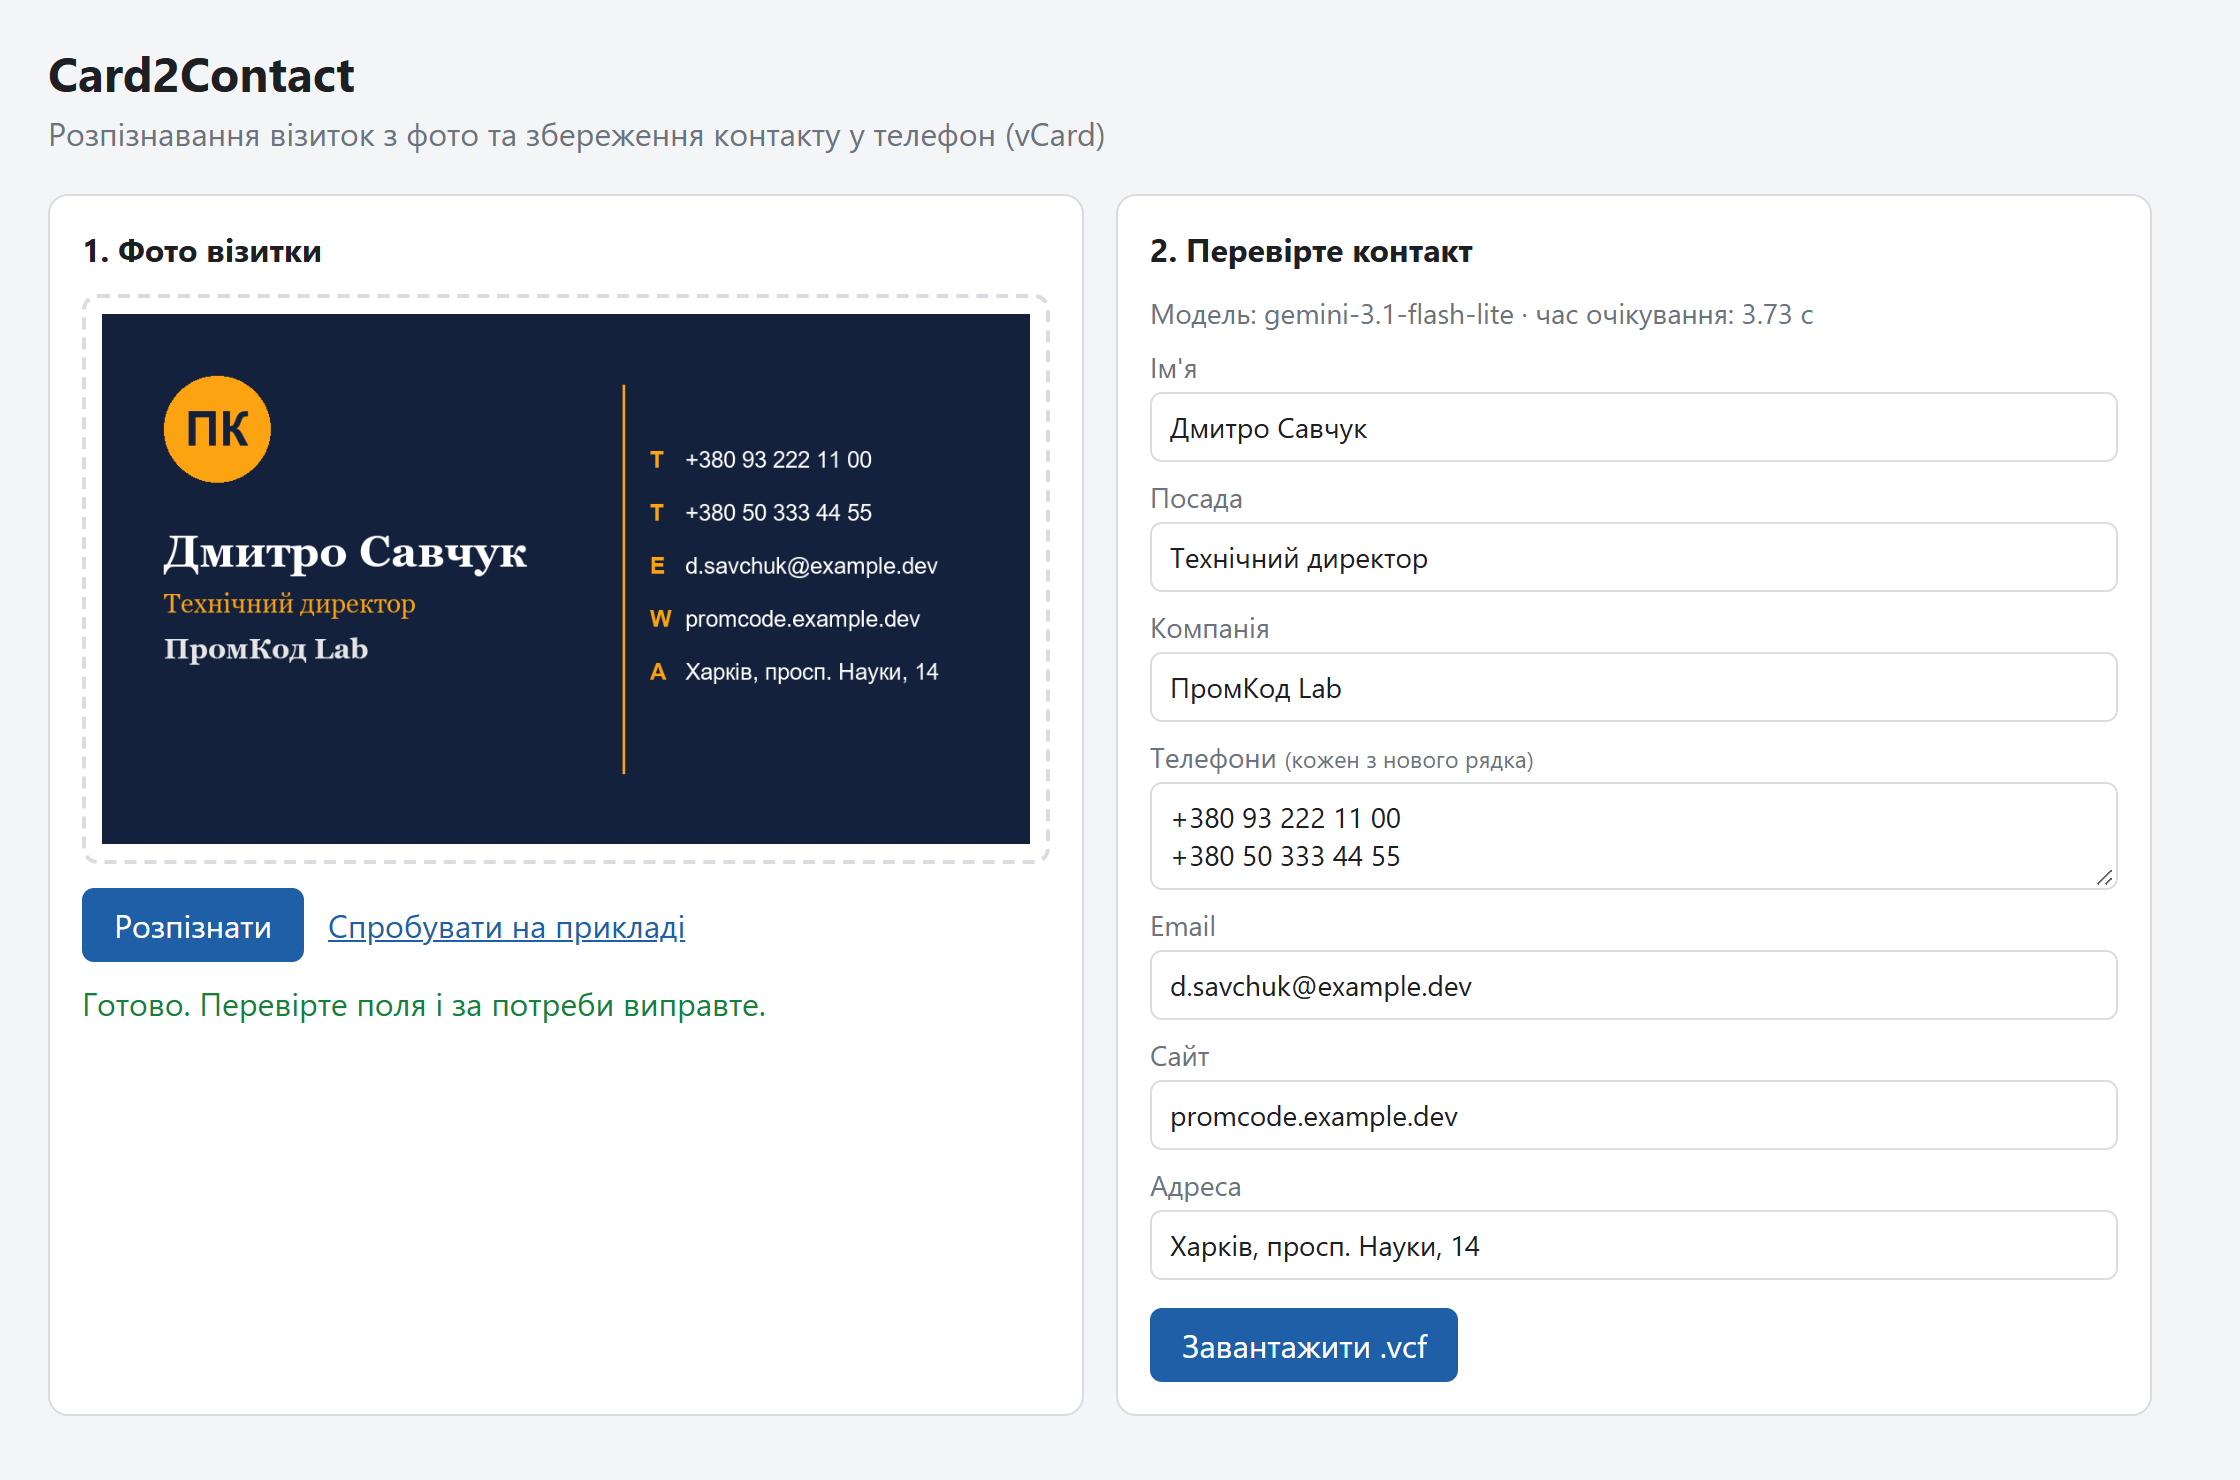
\includegraphics[width=\linewidth]{img/ui.png}
    \end{column}
    \begin{column}{0.38\textwidth}
      \begin{enumerate}
        \item Завантажити фото (drag-and-drop або вибір файлу).
        \item Натиснути «Розпізнати».
        \item Перевірити поля, за потреби виправити.
        \item «Завантажити .vcf» --- контакт імпортується в телефон.
      \end{enumerate}
      \medskip
      Кнопка «Спробувати на прикладі» --- демо без власного фото.
    \end{column}
  \end{columns}
\end{frame}

% ---------------------------------------------------------------- 9
\begin{frame}{Що вміє програма}
  \begin{itemize}
    \item Приймає JPG, PNG, WebP, HEIC --- до 10 МБ.
    \item Розпізнає 7 полів: ім'я, посада, компанія, телефони, email, сайт, адреса.
    \item Читає українські, англійські, польські, двомовні, рукописні візитки й фото під кутом.
    \item Приводить телефони до міжнародного формату (\code{044\ldots} $\to$ \code{+380 44\ldots}).
    \item Не вигадує: відсутні на візитці поля лишає порожніми.
    \item Три способи роботи: веб-інтерфейс, CLI, REST API
          (\code{POST /api/scan}, \code{POST /api/vcard}, Swagger \code{/docs}).
    \item Автоматичний перехід на запасну модель при 429 / 500 / 503 / 504.
  \end{itemize}
\end{frame}

% ---------------------------------------------------------------- 10
\begin{frame}{Чого не вміє}
  \begin{itemize}
    \item Одна візитка і одна її сторона за раз --- без пакетного режиму.
    \item Без історії запитів, акаунтів і автентифікації.
    \item Ім'я ділиться просто: останнє слово --- прізвище (порядок «Прізвище Ім'я» виправляють у формі).
    \item Адреса --- одним рядком, без розбиття на місто й індекс у vCard.
    \item Потрібен інтернет --- уся обробка в хмарі.
    \item Залежить від навантаження безкоштовного рівня: зазвичай 2--8 с,
          у пікові години моделі відповідають 503 / 429.
  \end{itemize}

  \summary{більшість обмежень --- свідомі спрощення прототипу, а не обмеження хмарного сервісу.}
\end{frame}

% ---------------------------------------------------------------- 11
\begin{frame}{Перевірка якості}
  6 синтетичних візиток (люди вигадані) з відомими правильними відповідями;
  скрипт \code{tools/evaluate.py} порівнює 7 полів.

  \medskip
  \centering
  \small
  \begin{tabular}{llccc}
    \toprule
    \textbf{Візитка} & \textbf{Особливість} & \textbf{Полів} & \textbf{Модель} & \textbf{Час, с} \\
    \midrule
    card\_uk & українська & 7/7 & 3.5-flash-lite & 2.1 \\
    card\_en & англійська, США & 7/7 & 3.5-flash-lite & 3.2 \\
    card\_dark & темний фон, логотип, 2 колонки & 7/7 & 3.5-flash-lite & 3.2 \\
    card\_photo & фото під кутом, розмите & 7/7 & 3.1-flash-lite & 3.5 \\
    card\_handwritten & рукописна, лише 3 поля & 7/7 & 3.5-flash-lite & 8.2 \\
    card\_vertical & вертикальна, двомовна & 7/7 & 3.5-flash-lite & 2.8 \\
    \bottomrule
  \end{tabular}
  \normalsize

  \raggedright
  \summary{42 з 42 полів. Час --- повне очікування користувача, разом зі спробами на зайнятих моделях.}
\end{frame}

% ---------------------------------------------------------------- 12
\begin{frame}{Скільки це коштує}
  Pay-as-you-go за токени (зображення теж перетворюється на токени).

  \medskip
  \centering
  \begin{tabular}{lL{0.33\textwidth}L{0.3\textwidth}}
    \toprule
     & \textbf{Безкоштовний tier} & \textbf{Платний tier} \\
    \midrule
    Ціна & 0 & частки цента за візитку \\
    Ліміт & запити на хвилину і на добу & значно вищі ліміти \\
    Банківська картка & не потрібна & потрібна \\
    Дані запитів & можуть покращувати продукти Google & не використовуються \\
    \bottomrule
  \end{tabular}

  \raggedright
  \summary{для прототипа безкоштовного рівня вистачає. Але за вечір тестів денна квота
  однієї моделі закінчилась --- для реальних користувачів потрібен платний рівень.}
\end{frame}

% ---------------------------------------------------------------- 13
\begin{frame}{Сфери застосування}
  \centering
  \begin{tabular}{ll}
    \toprule
    \textbf{Сфера} & \textbf{Приклади} \\
    \midrule
    Нетворкінг, конференції & стос візиток $\to$ контакти за хвилини \\
    Продажі, CRM & нові клієнти з візиток одразу в базу \\
    HR і рекрутинг & контакти кандидатів з ярмарків вакансій \\
    Малий бізнес & облік постачальників і партнерів \\
    Доступність & не треба вчитуватися в дрібний шрифт \\
    \bottomrule
  \end{tabular}

  \raggedright
  \summary{через відкритий API цю функцію можна вбудувати у власний продукт: CRM, месенджер, застосунок.}
\end{frame}

% ---------------------------------------------------------------- 14
\begin{frame}{Як розвинути в хмарі}
  \begin{itemize}
    \item \textbf{Cloud Run} --- Dockerfile вже є; автомасштабування 0 $\to$ N контейнерів.
    \item \textbf{Google People API} --- зберігати контакт одразу в Google Контакти.
    \item \textbf{Firebase Auth + Firestore} --- акаунти та історія відсканованих візиток.
    \item \textbf{Cloud Storage} --- зберігати фото візиток.
    \item \textbf{Pub/Sub або Cloud Tasks} --- черга для пакетного сканування стосу візиток.
    \item \textbf{Secret Manager} --- API-ключ замість файлу \code{.env}.
    \item \textbf{Vertex AI} --- для корпоративних даних: IAM, вибір регіону, SLA, аудит.
  \end{itemize}
\end{frame}

% ---------------------------------------------------------------- 15
\begin{frame}{Висновки}
  \begin{enumerate}
    \item Multimodal LLM замінює ланцюжок «OCR + власний парсер полів» одним API-викликом;
          JSON-схема робить відповідь передбачуваною.
    \item Python + FastAPI + HTML/JS --- робочий сервіс без власних моделей і GPU,
          уся AI-робота в хмарі Google.
    \item На 6 тестових візитках --- 42 з 42 полів; каскад моделей рятує від перевантаження (503 / 429).
    \item Проєкт --- приклад AIaaS: споживаємо готову модель через API, а не хостимо власну.
  \end{enumerate}

  \vspace{2.4em}
  \centering
  {\large Код: \code{https://github.com/tapa2/card2contact}}
\end{frame}

\end{document}
